% =====================================================================
%  OLV-6 — Corrections du rapport final (8 pages) suite aux remarques
%  Passages LaTeX prêts à coller. Chaque bloc indique OÙ le placer.
%  Figures : copier le dossier figures/ à côté du .tex principal.
%  Paquets supposés présents : graphicx, booktabs (sinon remplacer
%  \toprule/\midrule/\bottomrule par \hline).
% =====================================================================


% ---------------------------------------------------------------------
% [1] RÉSUMÉ — remplacer tout le paragraphe « Résumé — ... discutées. »
% ---------------------------------------------------------------------
Cette étude compare cinq approches de détection de disparition probable
d'oliviers à partir d'images satellitaires de 2019 à 2021 : seuil de
variation, CUSUM, Isolation Forest, réseau siamois convolutionnel
(Siamese CNN) et Temporal Convolutional Network (TCN). Sur OQDS, après
contrôle qualité, 71\,956 arbres sont répartis par blocs spatiaux de
250\,m en ensembles d'entraînement (51\,425), validation (10\,326) et
test (10\,205). Tous les choix (architecture, époque, seuil) sont faits
sur la validation par PR-AUC ; le test n'est évalué qu'une fois, après
gel des choix. Une version améliorée du réseau siamois (trois blocs
convolutifs avec normalisation, patches de 32$\times$32 pixels,
augmentation, arrêt anticipé, ensemble de 5 graines) atteint sur le test
une ROC-AUC de 0,961, une PR-AUC de 0,486 et un F1 de 0,482, avec un
rappel de 72,2\,\% (contre 0,874 / 0,220 / 0,322 et 34,6\,\% pour la
version initiale). Des intervalles de confiance par bootstrap spatial,
un contrôle de fuite de données et une étude d'ablation montrent que le
gain est réel mais que l'incertitude sur le test reste importante, les
positifs étant concentrés dans 5 blocs spatiaux. La cible demeure un
proxy de disparition et non un diagnostic sanitaire.


% ---------------------------------------------------------------------
% [2] NUMÉROTATION DES FIGURES — deux figures portent « Fig. 4 »
%     (« Pipeline expérimental » et « Principe du réseau siamois »).
%     Cause habituelle : une légende tapée à la main (\caption*{Fig. 4...}
%     ou texte sous l'image) au lieu de \caption{}. Utiliser partout :
% ---------------------------------------------------------------------
\begin{figure}[t]
  \centering
  \includegraphics[width=\linewidth]{pipeline.png} % votre fichier actuel
  \caption{Pipeline expérimental : mêmes arbres OQDS, sélection sur
           validation et test final figé.}
  \label{fig:pipeline}
\end{figure}
% ... et de même \caption{...}\label{fig:siamese} pour le schéma siamois.
% LaTeX renumérote alors toutes les figures automatiquement ; dans le
% texte, citer par \ref{fig:pipeline} au lieu d'écrire « Fig. 4 ».


% ---------------------------------------------------------------------
% [3] SECTION 4.4 — ajouter à la fin de « Deux réseaux profonds »
% ---------------------------------------------------------------------
\paragraph{Version améliorée du réseau siamois.}
Les courbes d'apprentissage de la première version montraient un
sous-apprentissage (PR-AUC de validation encore croissante à la fin de
l'entraînement). La version retenue (Siamese~v2, 84\,721 paramètres)
utilise trois blocs convolutifs avec normalisation par lots, des
patches de 32$\times$32 pixels (au lieu de 16$\times$16), une
augmentation géométrique identique pour les deux dates (rotations de
90°, symétries) et une variation radiométrique indépendante par date.
L'entraînement utilise AdamW, une entropie croisée pondérée par
$\sqrt{n_-/n_+}$, une réduction du pas d'apprentissage sur plateau et
un arrêt anticipé (patience 7, au plus 40 époques). Cinq graines sont
entraînées et leurs scores moyennés (ensemble).


% ---------------------------------------------------------------------
% [4] TABLE 1 (section 5.3) — ajouter cette ligne sous « Siamese CNN »
% ---------------------------------------------------------------------
% Siamese v2 & 8 & v2\_p32\_bce & lr$=10^{-3}$ ; largeur 16 ; dropout 0,30 ; patch 32 ; 5 graines & .3141 & .7185 \\
%
% Et ajouter à la légende de la Table 1 :
%   « Siamese v2 : PR-AUC de l'ensemble de 5 graines sur Validation. »


% ---------------------------------------------------------------------
% [5] TABLE 2 (section 6) — remplacer la table par celle-ci
% ---------------------------------------------------------------------
\begin{table*}[t]
\centering
\caption{Performances sur les 10\,205 arbres Test (seuils fixés sur
Validation). IC95 : intervalle de confiance à 95\,\% par bootstrap
de blocs spatiaux.}
\label{tab:test}
\small
\begin{tabular}{lccccccc}
\toprule
Modèle & Acc. & Préc. & Rappel & F1 & ROC-AUC & PR-AUC & IC95 PR-AUC \\
\midrule
\textbf{Siamese v2 (ensemble 5 graines)} & .964 & .362 & .722 & \textbf{.482} & \textbf{.961} & \textbf{.486} & [.110 ; .729] \\
Siamese CNN (initial)  & .966 & .301 & .346 & .322 & .874 & .220 & [.032 ; .442] \\
TCN                    & .719 & .055 & .692 & .103 & .763 & .062 & [.007 ; .147] \\
CUSUM                  & .913 & .047 & .143 & .071 & .652 & .039 & [.006 ; .090] \\
Seuil                  & .932 & .032 & .068 & .044 & .625 & .033 & [.005 ; .078] \\
Isolation Forest       & .407 & .027 & .692 & .051 & .556 & .026 & [.004 ; .057] \\
\bottomrule
\end{tabular}
\end{table*}


% ---------------------------------------------------------------------
% [6] SECTION 6.1 — remplacer « Modèle en tête : Siamese CNN »
% ---------------------------------------------------------------------
\subsection{Modèle en tête : Siamese v2}
Le Siamese v2 obtient les meilleurs F1, ROC-AUC et PR-AUC. Au seuil
fixé sur Validation, il retrouve 171 des 237 positifs (rappel
72,2\,\%) pour 302 fausses alertes (précision 36,2\,\%), contre 82
positifs retrouvés et 190 fausses alertes pour la version initiale.
Sur 5 graines, la PR-AUC Test vaut $0{,}468 \pm 0{,}050$ (version
initiale : $0{,}215 \pm 0{,}039$) : le gain ne dépend pas d'une graine
favorable. Le test apparié par bootstrap de blocs donne un gain de
PR-AUC de $+0{,}24$ (IC95 $[0{,}08 ; 0{,}35]$) sur le Siamese initial
et des gains significatifs sur toutes les autres méthodes. L'IC95 de la
PR-AUC reste toutefois large ($[0{,}11 ; 0{,}73]$), car les positifs du
test sont concentrés dans 5 des 52 blocs spatiaux.

\begin{figure}[t]
  \centering
  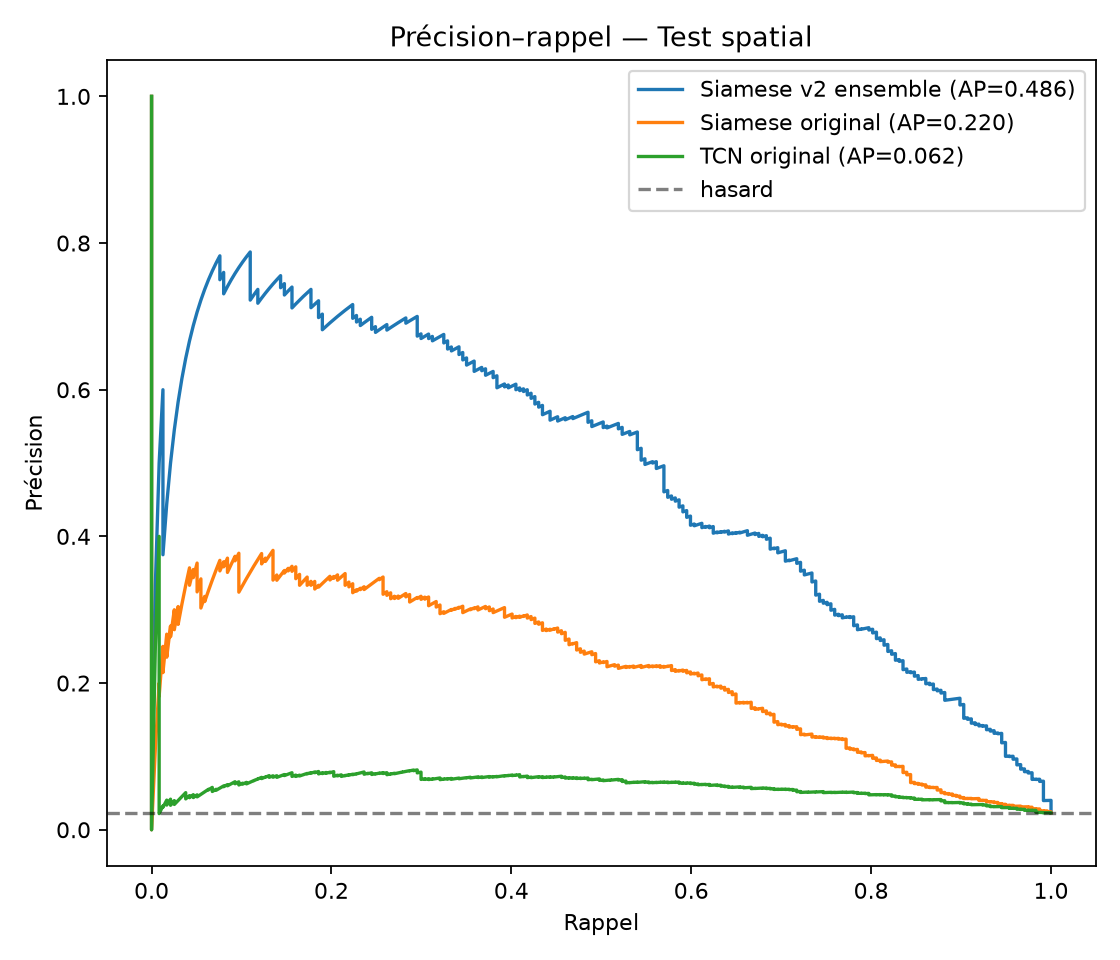
\includegraphics[width=\linewidth]{figures/pr_curves_original_vs_improved.png}
  \caption{Courbes précision-rappel sur Test : Siamese initial et
           Siamese v2.}
  \label{fig:pr_v2}
\end{figure}


% ---------------------------------------------------------------------
% [7] SECTION 6 — remplacer « Interprétation pratique » (comptes v2)
% ---------------------------------------------------------------------
\paragraph{Interprétation pratique.}
Le seuil se choisit selon la capacité d'inspection. Avec le Siamese v2,
inspecter les 2\,\% d'arbres les mieux classés retrouve 54,9\,\% des
positifs (une alerte sur deux est juste) ; à 5\,\%, 75,5\,\% des
positifs sont retrouvés avec 3,2 inspections par arbre réellement
disparu. Pour un rappel d'au moins 80\,\%, il faut inspecter 13,4\,\%
des arbres avec le Siamese v2, contre 30,8\,\% avec la version initiale
et 54,7\,\% avec le TCN.


% ---------------------------------------------------------------------
% [8] SECTION 7.1 — remplacer la première phrase (matrice de confusion)
% ---------------------------------------------------------------------
Le Siamese v2 produit 9\,666 vrais négatifs, 302 faux positifs, 66 faux
négatifs et 171 vrais positifs (version initiale : 9\,778 / 190 / 155 /
82). Le nombre d'omissions est divisé par 2,3, au prix de 112 alertes
supplémentaires.
% (La suite du paragraphe sur les hypothèses d'erreur peut rester.
%  Figure optionnelle : figures/examples_confusion_compact.png)


% ---------------------------------------------------------------------
% [9] NOUVELLE SECTION 7.4 — Robustesse et ablation (avant la section 8)
% ---------------------------------------------------------------------
\subsection{Contrôle de fuite et étude d'ablation}
\textbf{Fuite spatiale.} En retirant du test les arbres situés à moins
de 16, 32 ou 50\,m d'un arbre d'entraînement, la ROC-AUC reste stable
(0,955 à 0,965) et la PR-AUC rapportée à la prévalence reste de 21 à 24
fois le hasard ; à 100\,m, il ne reste que 13 positifs, effectif trop
faible pour conclure.
Un modèle ne voyant que l'image 2019 est au niveau du hasard (PR-AUC
$0{,}039$) : il n'existe pas de raccourci contextuel (sol, parcelle).

\textbf{Ablation.} Chaque variante est entraînée avec les mêmes
hyperparamètres et trois graines (Table~\ref{tab:ablation}). La
comparaison des deux dates apporte environ $+0{,}12$ à $+0{,}15$ de
PR-AUC par rapport à l'image 2021 seule, ce qui justifie l'architecture
siamoise. Le partage des poids donne la même performance avec deux fois
moins de paramètres. La couleur aide en validation ($-0{,}06$ en
niveaux de gris), sans effet net sur le test. L'ajout de l'image 2020
est la meilleure variante en validation ($0{,}368$ contre $0{,}297$)
comme en test ; elle est recommandée pour l'étape suivante.

\begin{table}[t]
\centering
\caption{Ablation du Siamese v2 : PR-AUC moyenne $\pm$ écart-type sur 3 graines.}
\label{tab:ablation}
\small
\begin{tabular}{lccc}
\toprule
Variante & Param. & Val. & Test \\
\midrule
Référence (2019+2021)       & 84\,721  & .297 $\pm$ .011 & .434 $\pm$ .017 \\
3 dates (2019+2020+2021)    & 88\,817  & .368 $\pm$ .031 & .484 $\pm$ .053 \\
Sans partage des poids      & 157\,025 & .297 $\pm$ .017 & .454 $\pm$ .085 \\
Niveaux de gris             & 84\,433  & .235 $\pm$ .013 & .446 $\pm$ .081 \\
Image 2021 seule            & 76\,529  & .175 $\pm$ .013 & .283 $\pm$ .043 \\
Image 2019 seule (contrôle) & 76\,529  & .037 $\pm$ .004 & .039 $\pm$ .005 \\
\bottomrule
\end{tabular}
\end{table}

\textbf{TCN.} Avec trois dates, le champ récepteur du TCN (7 pas)
couvre toute la série dès le premier bloc. Un MLP sur les mêmes 12
valeurs obtient une PR-AUC comparable ($0{,}052$ contre $0{,}058$) :
la convolution temporelle n'apporte rien sur une série aussi courte.


% ---------------------------------------------------------------------
% [10] SECTION 8.3 — remplacer entièrement « Choix pour la suite »
%      (l'ancienne version justifiait le choix par le TEST : erreur
%       méthodologique relevée par le jury)
% ---------------------------------------------------------------------
\subsection{Choix pour la suite}
Le choix du modèle repose uniquement sur la PR-AUC de Validation : le
Siamese v2 y obtient $0{,}314$ (ensemble), contre $0{,}167$ pour le
Siamese initial et $0{,}054$ au mieux pour les méthodes non
neuronales. Le test, évalué une seule fois après gel des choix, confirme
ce classement mais n'a pas servi à le produire. Le modèle accepte
directement deux images d'un même arbre, ce qui correspond au besoin
applicatif. Pour l'étape suivante, un service Python de prédiction
exposera le score, le seuil fixé et la version du checkpoint ; Spring
Boot consommera cette API. L'ajout de l'image 2020, meilleure variante
en validation lors de l'ablation, est la première amélioration prévue.
Un contrôle d'intensité simple reste utile comme référence explicable.


% ---------------------------------------------------------------------
% [11] SECTION 8.4 — remplacer « Limites et conclusion »
% ---------------------------------------------------------------------
\subsection{Limites et conclusion}
Cette étude mesure la disparition apparente de couronne et non un
diagnostic pathologique confirmé. Les images dites NDVI sont des rendus
RGB 8 bits non calibrés : un dépérissement sans disparition (couronne
présente mais affaiblie) n'est pas détectable dans ces conditions et
demanderait un canal proche infrarouge calibré. Le suivi ne couvre que
trois années, et l'incertitude sur le test reste forte (IC95 de la
PR-AUC entre 0,11 et 0,73) car les positifs sont concentrés dans peu de
blocs. Avec un rappel de 72\,\% pour une précision de 36\,\%, le
système est un outil de priorisation des inspections, pas un dispositif
de dépistage autonome. Une validation terrain indépendante (échantillon
d'alertes et de non-alertes vérifiées sur place, par drone ou visite)
et des images multispectrales calibrées sont nécessaires avant tout
usage réel.
